\documentclass[tikz]{standalone}

\usepackage{lmodern}
\usepackage{microtype}
\usepackage{amsfonts}
\usepackage{amsmath}
\usepackage{braket}

\usepackage{tikz}
\usetikzlibrary{calc, decorations, positioning}

\definecolor{googleB}{HTML}{4285F4}
\definecolor{googleG}{HTML}{34A853}
\definecolor{googleY}{HTML}{FBBC05}
\definecolor{googleR}{HTML}{EA4335}
\definecolor{googleBG}{HTML}{3B96A4}

% Main Document
\begin{document}
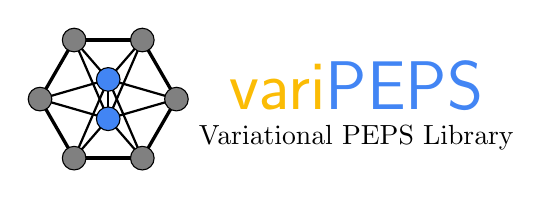
\begin{tikzpicture}
  \def\clipX{2.00}
  \def\clipY{1.75}
  \def\legLength{0.175}
  \def\tensorSize{0.15}
  \def\tensorShiftY{0.25}

  % ------------------------
  % triangular lattice sites
  % ------------------------

  \node at (3.15, 0.4\baselineskip) {\Huge\sffamily {\color{googleY}vari}{\color{googleB}PEPS}};
  \node at (3.15, -1.15\baselineskip) {\upshape Variational PEPS Library};

  % define coordinates for the triangular lattice
  \coordinate (T1) at ({+0.0*cos(30)}, {+0.0*cos(30)*tan(60)/2});

  \coordinate (C1) at ($(T1) + ({-0.5*cos(30)}, {+1.0*cos(30)*tan(60)/2})$);
  \coordinate (C2) at ($(T1) + ({+0.5*cos(30)}, {+1.0*cos(30)*tan(60)/2})$);
  \coordinate (C3) at ($(T1) + ({+1.0*cos(30)}, 0)$);
  \coordinate (C4) at ($(T1) + ({+0.5*cos(30)}, {-1.0*cos(30)*tan(60)/2})$);;
  \coordinate (C5) at ($(T1) + ({-0.5*cos(30)}, {-1.0*cos(30)*tan(60)/2})$);
  \coordinate (C6) at ($(T1) + ({-1.0*cos(30)}, 0)$);

  \draw[very thick] (C1) to (C2);
  \draw[very thick] (C2) to (C3);
  \draw[very thick] (C3) to (C4);
  \draw[very thick] (C4) to (C5);
  \draw[very thick] (C5) to (C6);
  \draw[very thick] (C6) to (C1);

  \draw[thick] ($(T1) + (0, +\tensorShiftY)$) to (C1);
  \draw[thick] ($(T1) + (0, -\tensorShiftY)$) to (C1);
  \draw[thick] ($(T1) + (0, +\tensorShiftY)$) to (C2);
  \draw[thick] ($(T1) + (0, -\tensorShiftY)$) to (C2);
  \draw[thick] ($(T1) + (0, +\tensorShiftY)$) to (C3);
  \draw[thick] ($(T1) + (0, -\tensorShiftY)$) to (C3);
  \draw[thick] ($(T1) + (0, +\tensorShiftY)$) to (C4);
  \draw[thick] ($(T1) + (0, -\tensorShiftY)$) to (C4);
  \draw[thick] ($(T1) + (0, +\tensorShiftY)$) to (C5);
  \draw[thick] ($(T1) + (0, -\tensorShiftY)$) to (C5);
  \draw[thick] ($(T1) + (0, +\tensorShiftY)$) to (C6);
  \draw[thick] ($(T1) + (0, -\tensorShiftY)$) to (C6);

  \begin{scope}[shift = {(T1)}]
    \begin{scope}[shift = {(0, +\tensorShiftY)}]
      % \draw[thick] (0,0) to ({-0.5*cos(30)}, {-1.0*cos(30)*tan(60)/2});
      % \draw[thick] ({+0.5*cos(30)}, {+1.0*cos(30)*tan(60)/2}) to (0, 0);
      % \draw[thick] ({-0.5*cos(30)}, {+1.0*cos(30)*tan(60)/2}) to (0, 0);
      % \draw[thick] (0, 0) to ({+0.5*cos(30)}, {-1.0*cos(30)*tan(60)/2});
      % \draw[thick] (0, 0) to ({-1.0*cos(30)}, 0);
      % \draw[thick] ({+1.0*cos(30)}, 0) to (0, 0);
      \draw[thick] (0, 0) to (0, -\tensorShiftY);
      \draw[black, fill = googleB] (0, 0) circle (\tensorSize);
    \end{scope}
    \begin{scope}[shift = {(0, -\tensorShiftY)}]
      % \draw[thick] (0,0) to ({-0.5*cos(30)}, {-1.0*cos(30)*tan(60)/2});
      % \draw[thick] ({+0.5*cos(30)}, {+1.0*cos(30)*tan(60)/2}) to (0, 0);
      % \draw[thick] ({-0.5*cos(30)}, {+1.0*cos(30)*tan(60)/2}) to (0, 0);
      % \draw[thick] (0, 0) to ({+0.5*cos(30)}, {-1.0*cos(30)*tan(60)/2});
      % \draw[thick] (0, 0) to ({-1.0*cos(30)}, 0);
      % \draw[thick] ({+1.0*cos(30)}, 0) to (0, 0);
      \draw[thick] (0, 0) to (0, +\tensorShiftY);
      \draw[black, fill = googleB] (0, 0) circle (\tensorSize);
    \end{scope}
  \end{scope}

  \foreach \tensor in {C1, C2, C3, C4, C5, C6} {
    \begin{scope}[shift = {(\tensor)}]
      \draw[black, fill = gray] (0, 0) circle (\tensorSize);
    \end{scope}
  }
\end{tikzpicture}
\end{document}

%%% Local Variables:
%%% mode: latex
%%% TeX-master: t
%%% End:
